\section{Funzionalit\`a offerte}
L'applicazione prevede la presenza di un Wallet associato a ciascun tenant, che pu\`o essere ricaricato tramite pagamenti effettuati con \textit{Stripe}.
All'interno del sistema sono previsti dei \textit{workflow}, processi che utilizzano dati provenienti da banche dati esterne per effettuare analisi di vario tipo.
Ogni operazione all'interno del workflow ha un costo, e per ognuna di queste viene scalato un determinato importo in base a un listino prezzi associato al tenant di appartenenza dell'utente.
Quando un'operazione viene inserita nella coda pagamenti, questa viene registrata nel database e il relativo importo viene scalato automaticamente dal Wallet del tenant.

In questo capitolo descriveremo descriveremo le interfacce e faremo alcune considerazioni sulla scelta della piattaforma di pagamento per le ricariche.
Parleremo degli altri requisiti funzionali pi\`u in dettaglio nei prossimi capitoli.\\\\
All'interno dell'interfaccia devono essere presenti due schermate, una per la gestione del Wallet e una per la gestione dei listini prezzi.

\section{Sezione gestione Wallet}
L'utente ha a disposizione una dashboard per monitorare il Wallet del suo tenant di appartenenza in cui pu\`o visualizzare lo storico delle transazioni e ricaricare il Wallet.

\begin{figure}[H]
  \centering
  \includegraphics[width=14cm]{images/gestione-wallet/mock-gestione-wallet.png}
  \caption{Wireframe della schermata di Gestione Wallet}
\end{figure}

Nella parte superiore abbiamo dei widget che riportano alcune informazioni in modo da essere facilmente accessibili:
\begin{enumerate}
  \item Credito disponibile
  \item Credito speso, con andamento in relazione al mese precedente
  \item Credito depositato, con andamento in relazione al mese precedente
  \item Differenza tra credito speso e credito depositato, con andamento in relazione al mese precedente.
\end{enumerate}

Il bottone \textit{Ricarica} apre una schermata che ti permette di caricare un importo arbitrario nel Wallet:

\begin{figure}[H]
  \centering
  % \includegraphics[width=8.5cm]{images/mock-gestione-wallet.png}
  \caption{Wireframe della schermata di selezione importo }
\end{figure}

Andando avanti si conferma l'importo e si passa alla schermata di pagamento di Stripe

\begin{figure}[H]
  \centering
  % \includegraphics[width=8.5cm]{images/mock-gestione-wallet.png}
  \caption{Wireframe della schermata di pagamento con Stripe }
\end{figure}

Il bottone \textit{Filtri} apre una schermata laterale in cui \`e possibile selezionare le propriet\`a per cui deve venire filtrata la lista delle transazioni.

\begin{figure}[H]
  \centering
  % \includegraphics[width=8.5cm]{images/mock-gestione-wallet.png}
  \caption{Wireframe della schermata dei filtri}
\end{figure}

\section{Sezione gestione listini prezzi}

\section{Considerazioni metodi di pagamento}
